\documentclass[11pt]{article}

\usepackage[margin=1in]{geometry}
\usepackage{graphicx}
\usepackage{booktabs}
\usepackage{amsmath}
\usepackage[hidelinks]{hyperref}
\usepackage{caption}
\usepackage{subcaption}

\title{3D Immersed-Boundary Cylinder: Preliminary Findings}
\author{3dRotatingCylinder Project}
\date{\today}

\begin{document}
\maketitle

\section{Overview}

These simulations model a rigid circular cylinder, free to translate in a
viscous fluid under gravity, while being driven by a prescribed oscillatory
cross-flow velocity. The cylinder is extruded along $z$ with periodic
boundary conditions in that direction, so the flow is effectively
three-dimensional only through whatever spanwise structure the body
introduces. The question this preliminary set of runs addresses is simple:
\emph{does adding radial fins along the cylinder's span change how it glides
through the fluid, relative to a bare cylinder?}

Four cases form a matched comparison, differing only in the number of fins
(0, 1, 2, or 3) attached at evenly spaced points along the span, with
identical fluid properties, domain, grid, and forcing:
\texttt{faster\_nofin\_full\_span}, \texttt{faster\_midfin},
\texttt{faster\_2fin}, and \texttt{faster\_3fin}. Two earlier cases,
\texttt{faster\_nofin} and \texttt{faster\_nofin\_large}, established the
baseline bare-cylinder behavior and motivated the larger domain used by the
fin series. A separate case, \texttt{endcaps}, tests end discs rather than
fins and uses different flow parameters, so it is not part of the controlled
comparison.

All reported trajectories, glide angles, and status data are transferred
from the hand-written \texttt{README.md} in each case's directory and from
the project's case index; see the project repository for the full narrative
and regeneration instructions.

\section{Case setups}

\subsection{Common parameters (fin series)}

\texttt{faster\_nofin\_full\_span}, \texttt{faster\_midfin},
\texttt{faster\_2fin}, and \texttt{faster\_3fin} share the following setup:

\begin{itemize}
  \item \textbf{Body:} solid circular cylinder, radius $R = 3.17$
        (diameter $D = 6.34$), axis along $z$, length $L = 35.0$ (spans the
        full periodic $z$-domain).
  \item \textbf{Fluid:} $\rho = 1.0$, $\mu = 0.01$, giving
        $\mathrm{Re} = \rho U D / \mu \approx 634$ based on diameter.
  \item \textbf{Domain:} $x \in [-30, 120]$, $y \in [-120, 30]$,
        $z \in [-17.5, 17.5]$; periodic in $z$.
  \item \textbf{Grid:} $150 \times 150 \times 35$ base grid, 4 AMR levels
        (refinement $4\cdot4\cdot2$), finest spacing $\Delta x = 0.0625$.
  \item \textbf{Forcing:} prescribed cross-flow velocity
        $U_\infty \cos(2\pi f t)$, $U = 1.0$, $f = 0.6$
        (Keulegan--Carpenter number $U/(fD) \approx 0.26$).
  \item \textbf{Buoyancy:} neutrally buoyant body ($\rho_\text{solid} =
        \rho_\text{fluid}$), net body force from a reduced gravity term
        ($\delta = 0.011$) active from $t = 0$, giving the cylinder a
        downward glide as it oscillates.
  \item \textbf{Run length:} target $\mathrm{END\_TIME} = 30$ (some cases
        were restarted past this; see Section~\ref{sec:findings}).
\end{itemize}

The immersed-boundary point cloud and the Eulerian grid are tied together:
the point spacing implied by each case's body parameters must equal the
finest Eulerian grid spacing above ($\Delta x = 0.0625$), or the one-point-
per-finest-cell assumption the IB method relies on is violated. This is a
modeling invariant across every case in this report, not something tuned
per case.

The cases differ only in how many fins are attached and where:

\begin{table}[h]
\centering
\begin{tabular}{@{}lccl@{}}
\toprule
Case & Fins & $z$-positions (fraction of span) & IB points \\
\midrule
\texttt{faster\_nofin\_full\_span} & 0 & --- & 4{,}524{,}800 \\
\texttt{faster\_midfin}            & 1 & $1/2$ & 4{,}549{,}032 \\
\texttt{faster\_2fin}              & 2 & $1/4,\ 3/4$ & 4{,}573{,}264 \\
\texttt{faster\_3fin}              & 3 & $1/6,\ 1/2,\ 5/6$ & 4{,}597{,}496 \\
\bottomrule
\end{tabular}
\caption{The fin series. Each fin has radius $2R = 6.34$, i.e.\ twice the
cylinder's own radius.}
\end{table}

\texttt{faster\_midfin} is the single-fin case: one fin at the axial
midpoint. \texttt{faster\_2fin} and \texttt{faster\_3fin} add fins
symmetrically outward from there.

\subsection{Baseline series}

\texttt{faster\_nofin} is the original bare-cylinder baseline: the same
cylinder (but shorter, $L = 25.5$, non-periodic $z$) in a smaller domain
($x \in [-20,80]$, $y \in [-72,18]$). Its first run exited the domain at
$t = 21.55$ when the body's center of mass approached the lower $y$
boundary. \texttt{faster\_nofin\_large} repeats it with the domain enlarged
to $x \in [-30,120]$, $y \in [-120,30]$ (the same size later reused by the
fin series) and completed the full run. The fin series uses this larger
domain, plus a longer, periodic-$z$ body so the cylinder is uniform across
its whole span.

\subsection{\texttt{endcaps} (not part of the controlled comparison)}

\texttt{endcaps} adds two discs (radius 7.0) capping the ends of a
\texttt{faster\_nofin}-sized cylinder, with no fins along the span. It also
changes the oscillation frequency ($f = 0.333$ vs.\ $0.6$), gravity onset
($t = 3.0$ vs.\ $t = 0$), and the upper-$y$ boundary condition (closed vs.\
open) relative to \texttt{faster\_nofin}, so it cannot be read as an
isolated effect of end geometry.

\section{Findings}
\label{sec:findings}

\subsection{Run status}

\begin{table}[h]
\centering
\small
\begin{tabular}{@{}lp{6.5cm}cc@{}}
\toprule
Case & Status & $t_\text{end}$ & Final COM $(x, y)$ \\
\midrule
\texttt{faster\_nofin} & domain exit & 21.5 & $(63.9, -67.5)$ \\
\texttt{faster\_nofin\_large} & complete & 30 & $(92.9, -92.8)$ \\
\texttt{faster\_nofin\_full\_span} & complete & 60 & $(112.5, -31.5)$ \\
\texttt{faster\_3fin} & crashed --- insufficient ghost cells near the
  physical boundary & 49.0 & $(112.3, -23.7)$ \\
\texttt{faster\_2fin} & timed out at the 72h wall-clock limit & 51.5 &
  $(110.7, -29.4)$ \\
\texttt{faster\_midfin} & crashed --- same ghost-cell error as
  \texttt{faster\_3fin} & 57.2 & $(112.6, -31.8)$ \\
\bottomrule
\end{tabular}
\caption{Status of each case as of the latest recorded run. Source:
project case index.}
\end{table}

\textbf{All three finned cases stall in the same place:} every one of
\texttt{faster\_midfin}, \texttt{faster\_2fin}, and \texttt{faster\_3fin}
reaches $x \approx 110$--$113$, close to the domain's $x_\text{max} = 120$,
before crashing or timing out. The two crashes are the identical failure
mode (an IB spreading operator running out of ghost cells once the body
gets close enough to the physical boundary); the timeout case is still
drifting toward the same region when its wall-clock budget runs out. This
is consistent across all three finned cases and looks like a boundary
proximity problem rather than anything specific to a given fin count ---
the bare-cylinder case in the same domain, \texttt{faster\_nofin\_full\_span},
reaches almost the same $x$ ($112.5$) but completes cleanly, which narrows
the likely cause to the fins' wider IB stencil needing more ghost-cell
width near the wall, not the boundary width itself.

\textbf{Note on data provenance:} the committed \texttt{faster\_nofin\_full\_span}
and \texttt{faster\_3fin} case READMEs still describe earlier, incomplete
attempts (an out-of-memory crash at $t=22.9$ for the former, a still-running
job at $t=29.1$ for the latter) that predate the final results in the table
above; those per-case write-ups were not updated after later, further
restarts. The table above reflects the most recent recorded state.

\subsection{Center-of-mass trajectories}

Figure~\ref{fig:trajectories} overlays the center-of-mass path of every case
with simulation output on one coordinate frame. The plotting convention:
for each case, whichever run reached furthest is shown --- a same-folder
restart (resumed from checkpoint) is stitched onto its earlier data as one
continuous line, while a fresh restart in a new run folder only replaces
the earlier line once its own reach exceeds it. The red dashed box is the
fin series' computational domain ($x \in [-30,120]$, $y \in [-120,30]$);
the purple dotted box is a smaller $100\times45$ reference domain
($x \in [-20,80]$, $y \in [-27,18]$) shown for scale.

\begin{figure}[h]
\centering
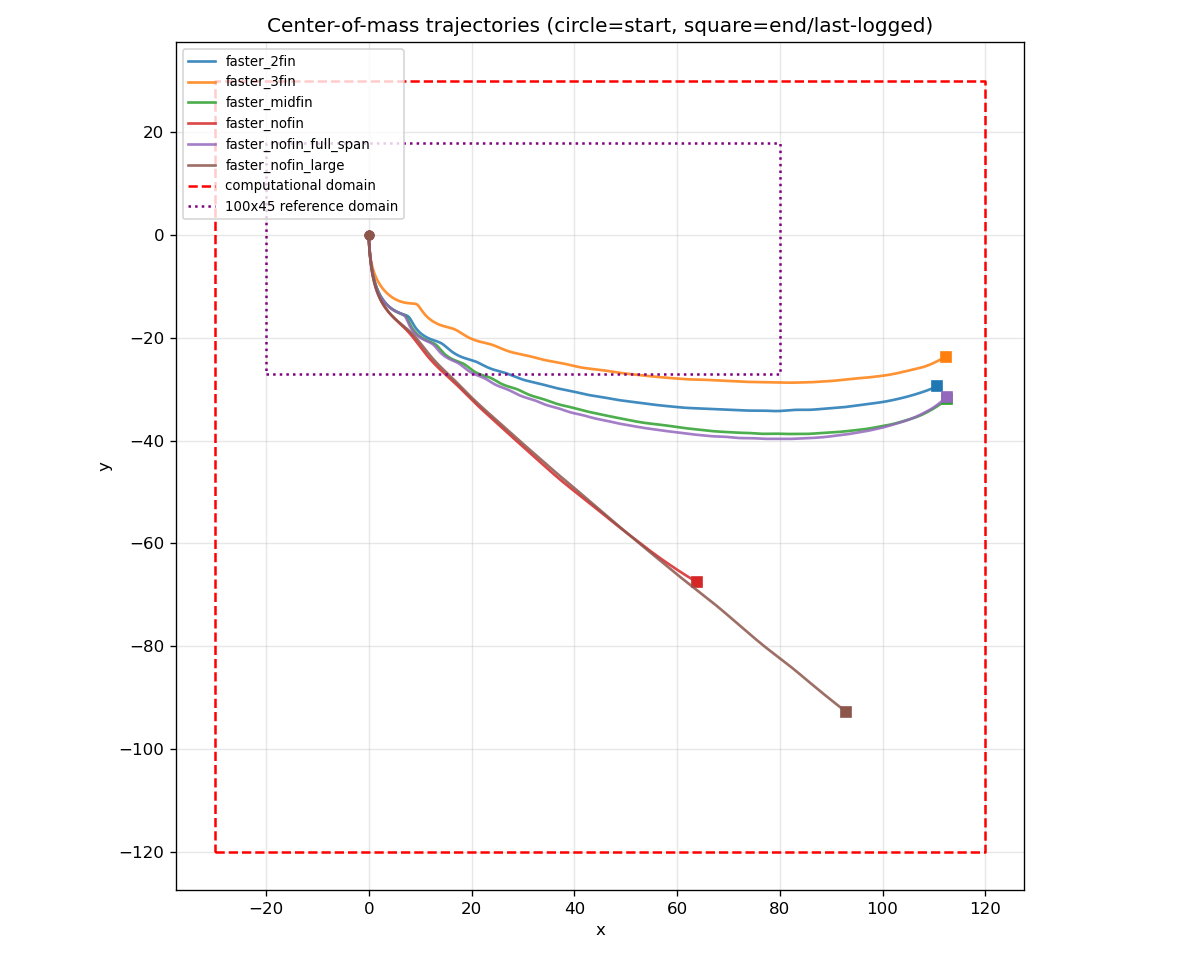
\includegraphics[width=0.85\linewidth]{figures/trajectory_comparison.png}
\caption{Center-of-mass trajectories for every case with simulation output
(circle = start, square = end / last logged point). Source: project case
index.}
\label{fig:trajectories}
\end{figure}

The two bare-cylinder baseline cases, \texttt{faster\_nofin} and
\texttt{faster\_nofin\_large}, fall almost on top of each other on a steep,
nearly straight path down to $y \approx -67$ to $-93$ before their runs end.
Every other case --- \texttt{faster\_nofin\_full\_span} and all three
finned cases --- peels away from that steep path much earlier and curves
into a much shallower descent, ending in a band around
$y \approx -24$ to $-39$ at $x \approx 110$--$113$. Within that band,
\texttt{faster\_3fin} (orange) sits clearly highest/flattest, with
\texttt{faster\_2fin}, \texttt{faster\_midfin}, and
\texttt{faster\_nofin\_full\_span} bunched lower and close together. That
last point is worth being careful about: because all four of those cases
were stopped at close to the same $x$ (the ghost-cell boundary issue in
Section~\ref{sec:findings} above), their similar endpoints may partly just
reflect being cut off at a similar point along a still-evolving curve,
rather than four cases that have each reached a converged glide angle.

\subsection{Effect of fins on glide angle}

Where glide-angle data is available, adding fins flattens the trajectory
substantially. The bare-cylinder cases settle into a glide angle (measured
from horizontal) of roughly $39^\circ$--$42^\circ$ once their trajectory
stabilizes (\texttt{faster\_nofin\_large}, steady by $t\approx20$). The
early, uninterrupted run of \texttt{faster\_3fin} (job 14817768, reaching
$t=29.1$ before later restarts) shows the glide angle dropping steadily
from $48.2^\circ$ at $t=2$--$3$ to just $2.5^\circ$ by $t=26$--$29$ ---
the body is moving almost horizontally by the end of that run, a
qualitatively different trajectory shape from the bare cylinder, and the
one case where the flattening is backed by a full time series rather than
just a final position. No comparably detailed glide-angle series was
committed for \texttt{faster\_midfin} or \texttt{faster\_2fin}; the
trajectory plot above (Figure~\ref{fig:trajectories}) shows both of them
also flattening relative to the bare cylinder, but --- per the caveat above
--- not by how much more than \texttt{faster\_nofin\_full\_span}, itself
finless, does over the same stretch. So whether the flattening effect
scales with fin count (1 vs.\ 2 vs.\ 3), or is mostly a 0-vs-any-fins
effect, is not yet established from the current data.

\subsection{Flow structure: bare cylinder vs.\ one fin}

Figures~\ref{fig:tube} and~\ref{fig:front} compare instantaneous vorticity
($\omega_z = \pm1$) iso-surfaces for \texttt{faster\_nofin\_full\_span} (no
fins) and \texttt{faster\_midfin} (one central fin) at $t \approx 22$, from
two camera angles: looking obliquely down the body's spanwise axis
(Figure~\ref{fig:tube}), and looking along the streamwise direction, into
the cross-flow/spanwise plane (Figure~\ref{fig:front}).

The bare cylinder sheds a comparatively regular, coiled wake that is
uniform along the span -- consistent with there being nothing to break the
spanwise symmetry. The single fin visibly disrupts this: the vorticity
surface folds and knots around the fin location, and an additional
elongated, less-structured wake is thrown off along the body axis
near the fin itself, where the bare cylinder has no comparable feature. This
is a qualitative confirmation, at the flow-structure level, of the same
effect the glide-angle numbers point to -- the fin is a significant local
perturbation to the wake, not a minor one.

\begin{figure}[p]
\centering
\begin{subfigure}{0.48\textwidth}
  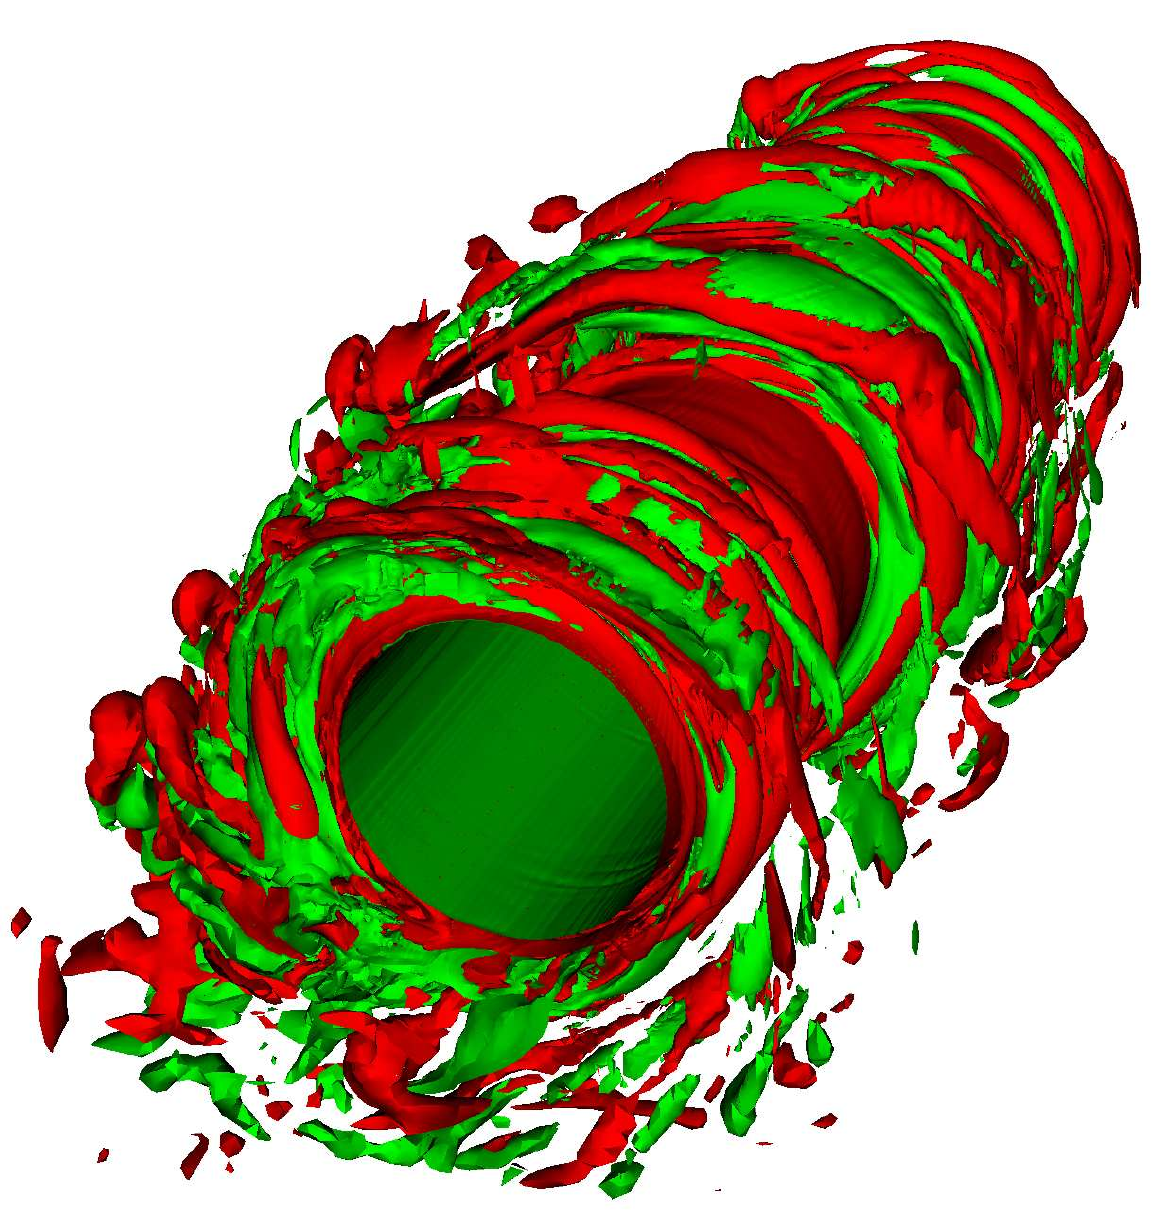
\includegraphics[width=\linewidth]{figures/faster_nofin_full_span_omega_z_t22_tube.png}
  \caption{\texttt{faster\_nofin\_full\_span} (0 fins)}
\end{subfigure}
\hfill
\begin{subfigure}{0.48\textwidth}
  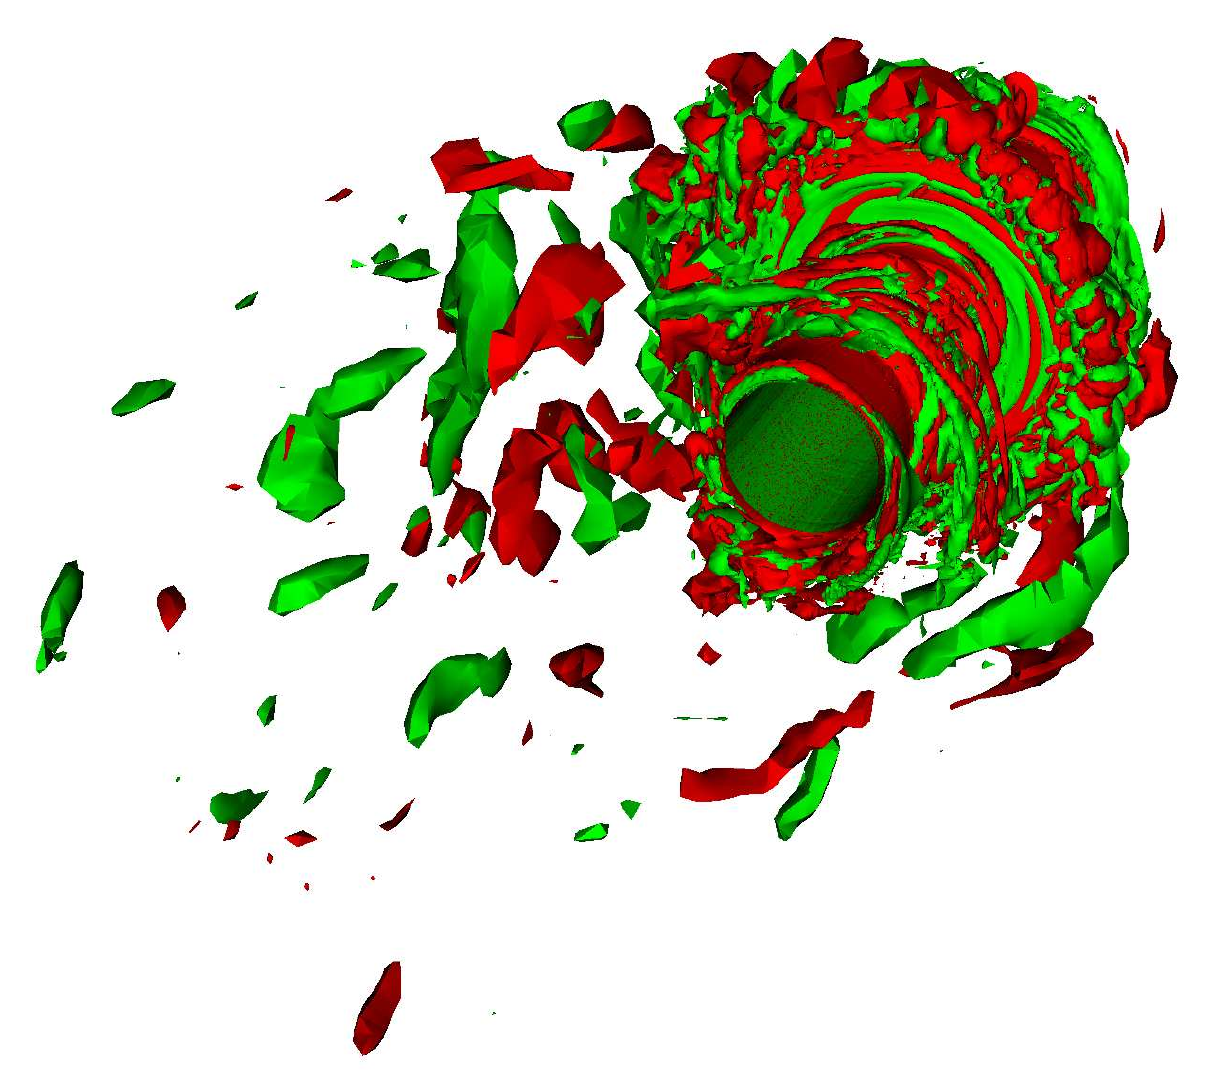
\includegraphics[width=\linewidth]{figures/faster_midfin_omega_z_t22_tube.png}
  \caption{\texttt{faster\_midfin} (1 fin)}
\end{subfigure}
\caption{Vorticity iso-surfaces ($\omega_z = \pm 1$; red $= -1$, green
$= +1$) at $t \approx 22$, viewed obliquely down the body's spanwise axis.}
\label{fig:tube}
\end{figure}

\begin{figure}[p]
\centering
\begin{subfigure}{0.48\textwidth}
  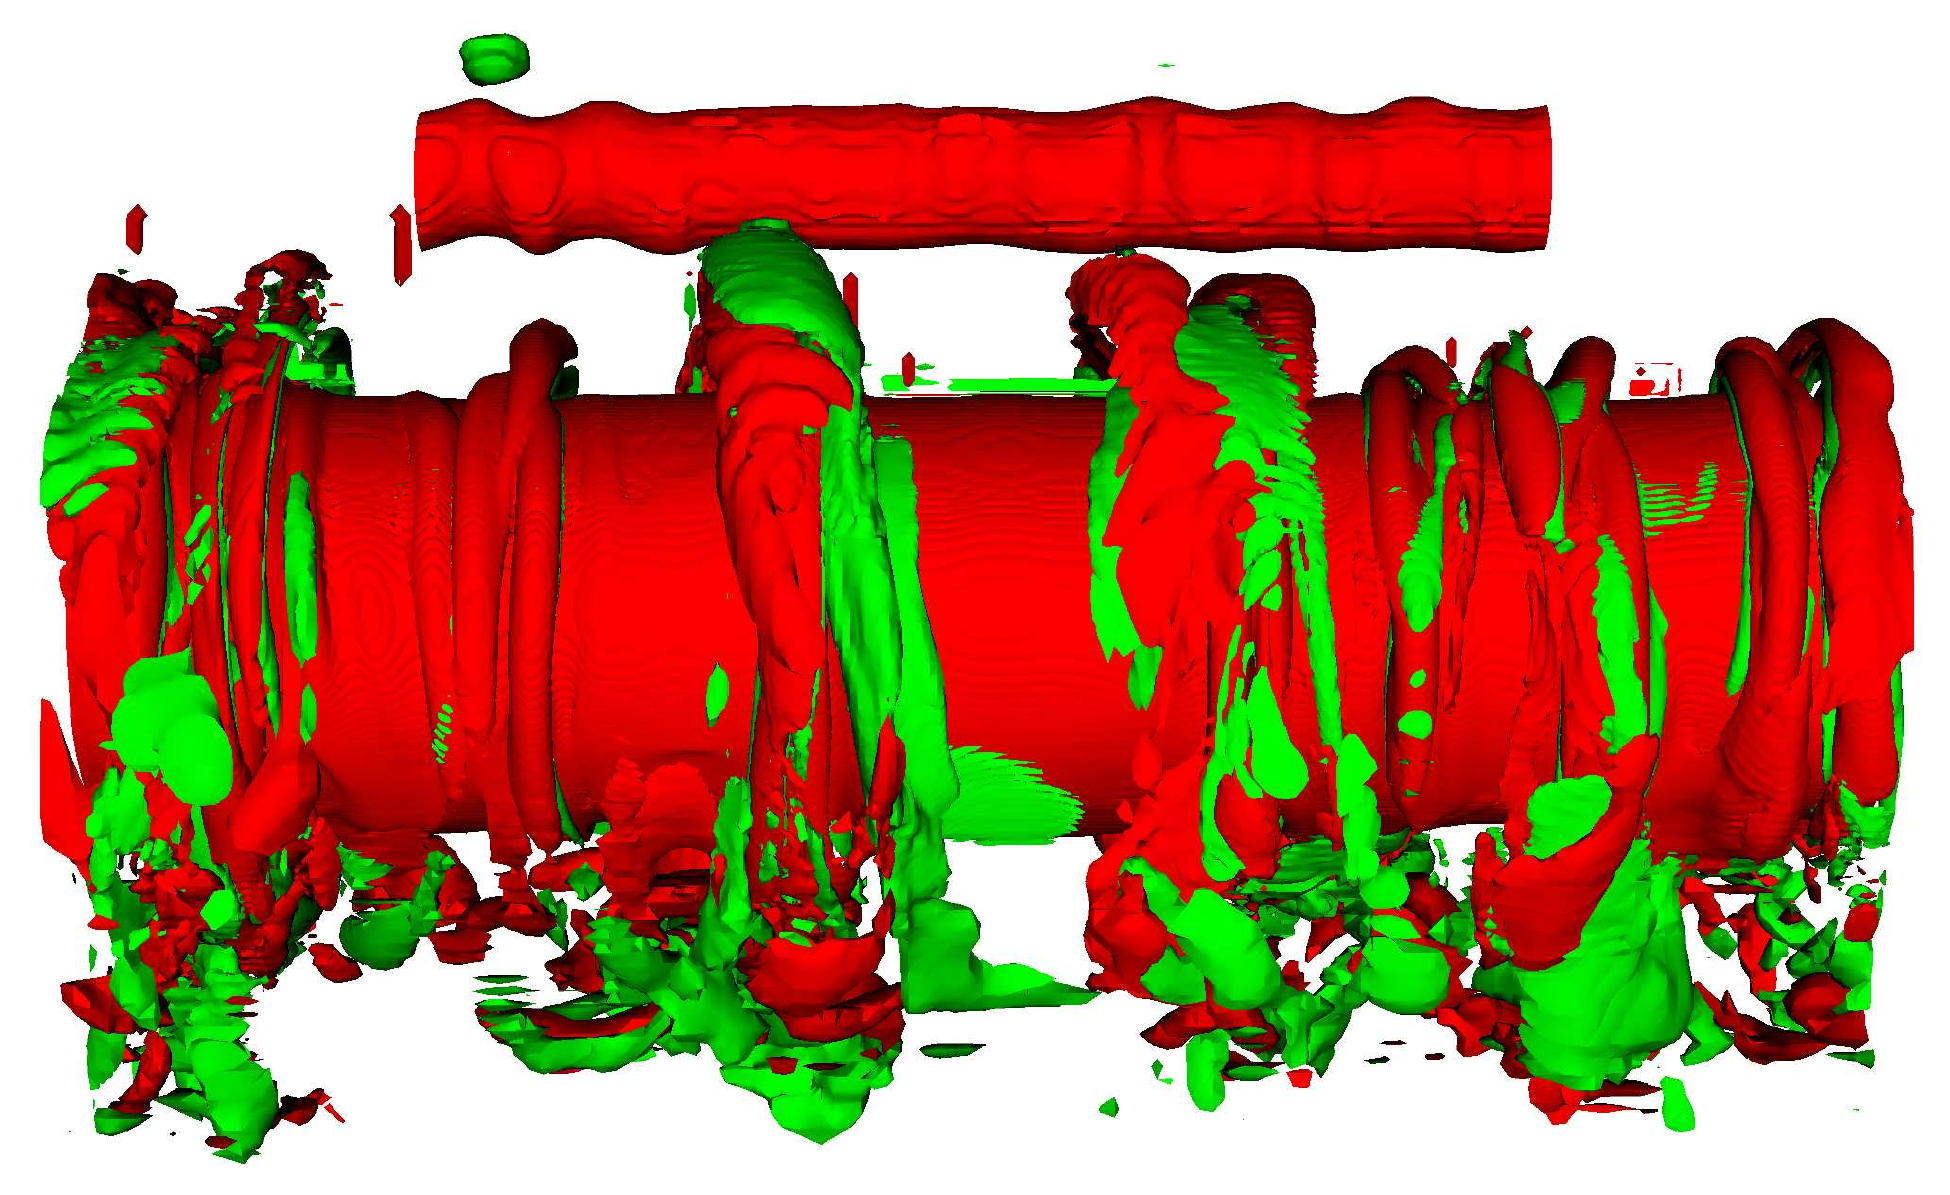
\includegraphics[width=\linewidth]{figures/faster_nofin_full_span_omega_z_t22_front.png}
  \caption{\texttt{faster\_nofin\_full\_span} (0 fins)}
\end{subfigure}
\hfill
\begin{subfigure}{0.48\textwidth}
  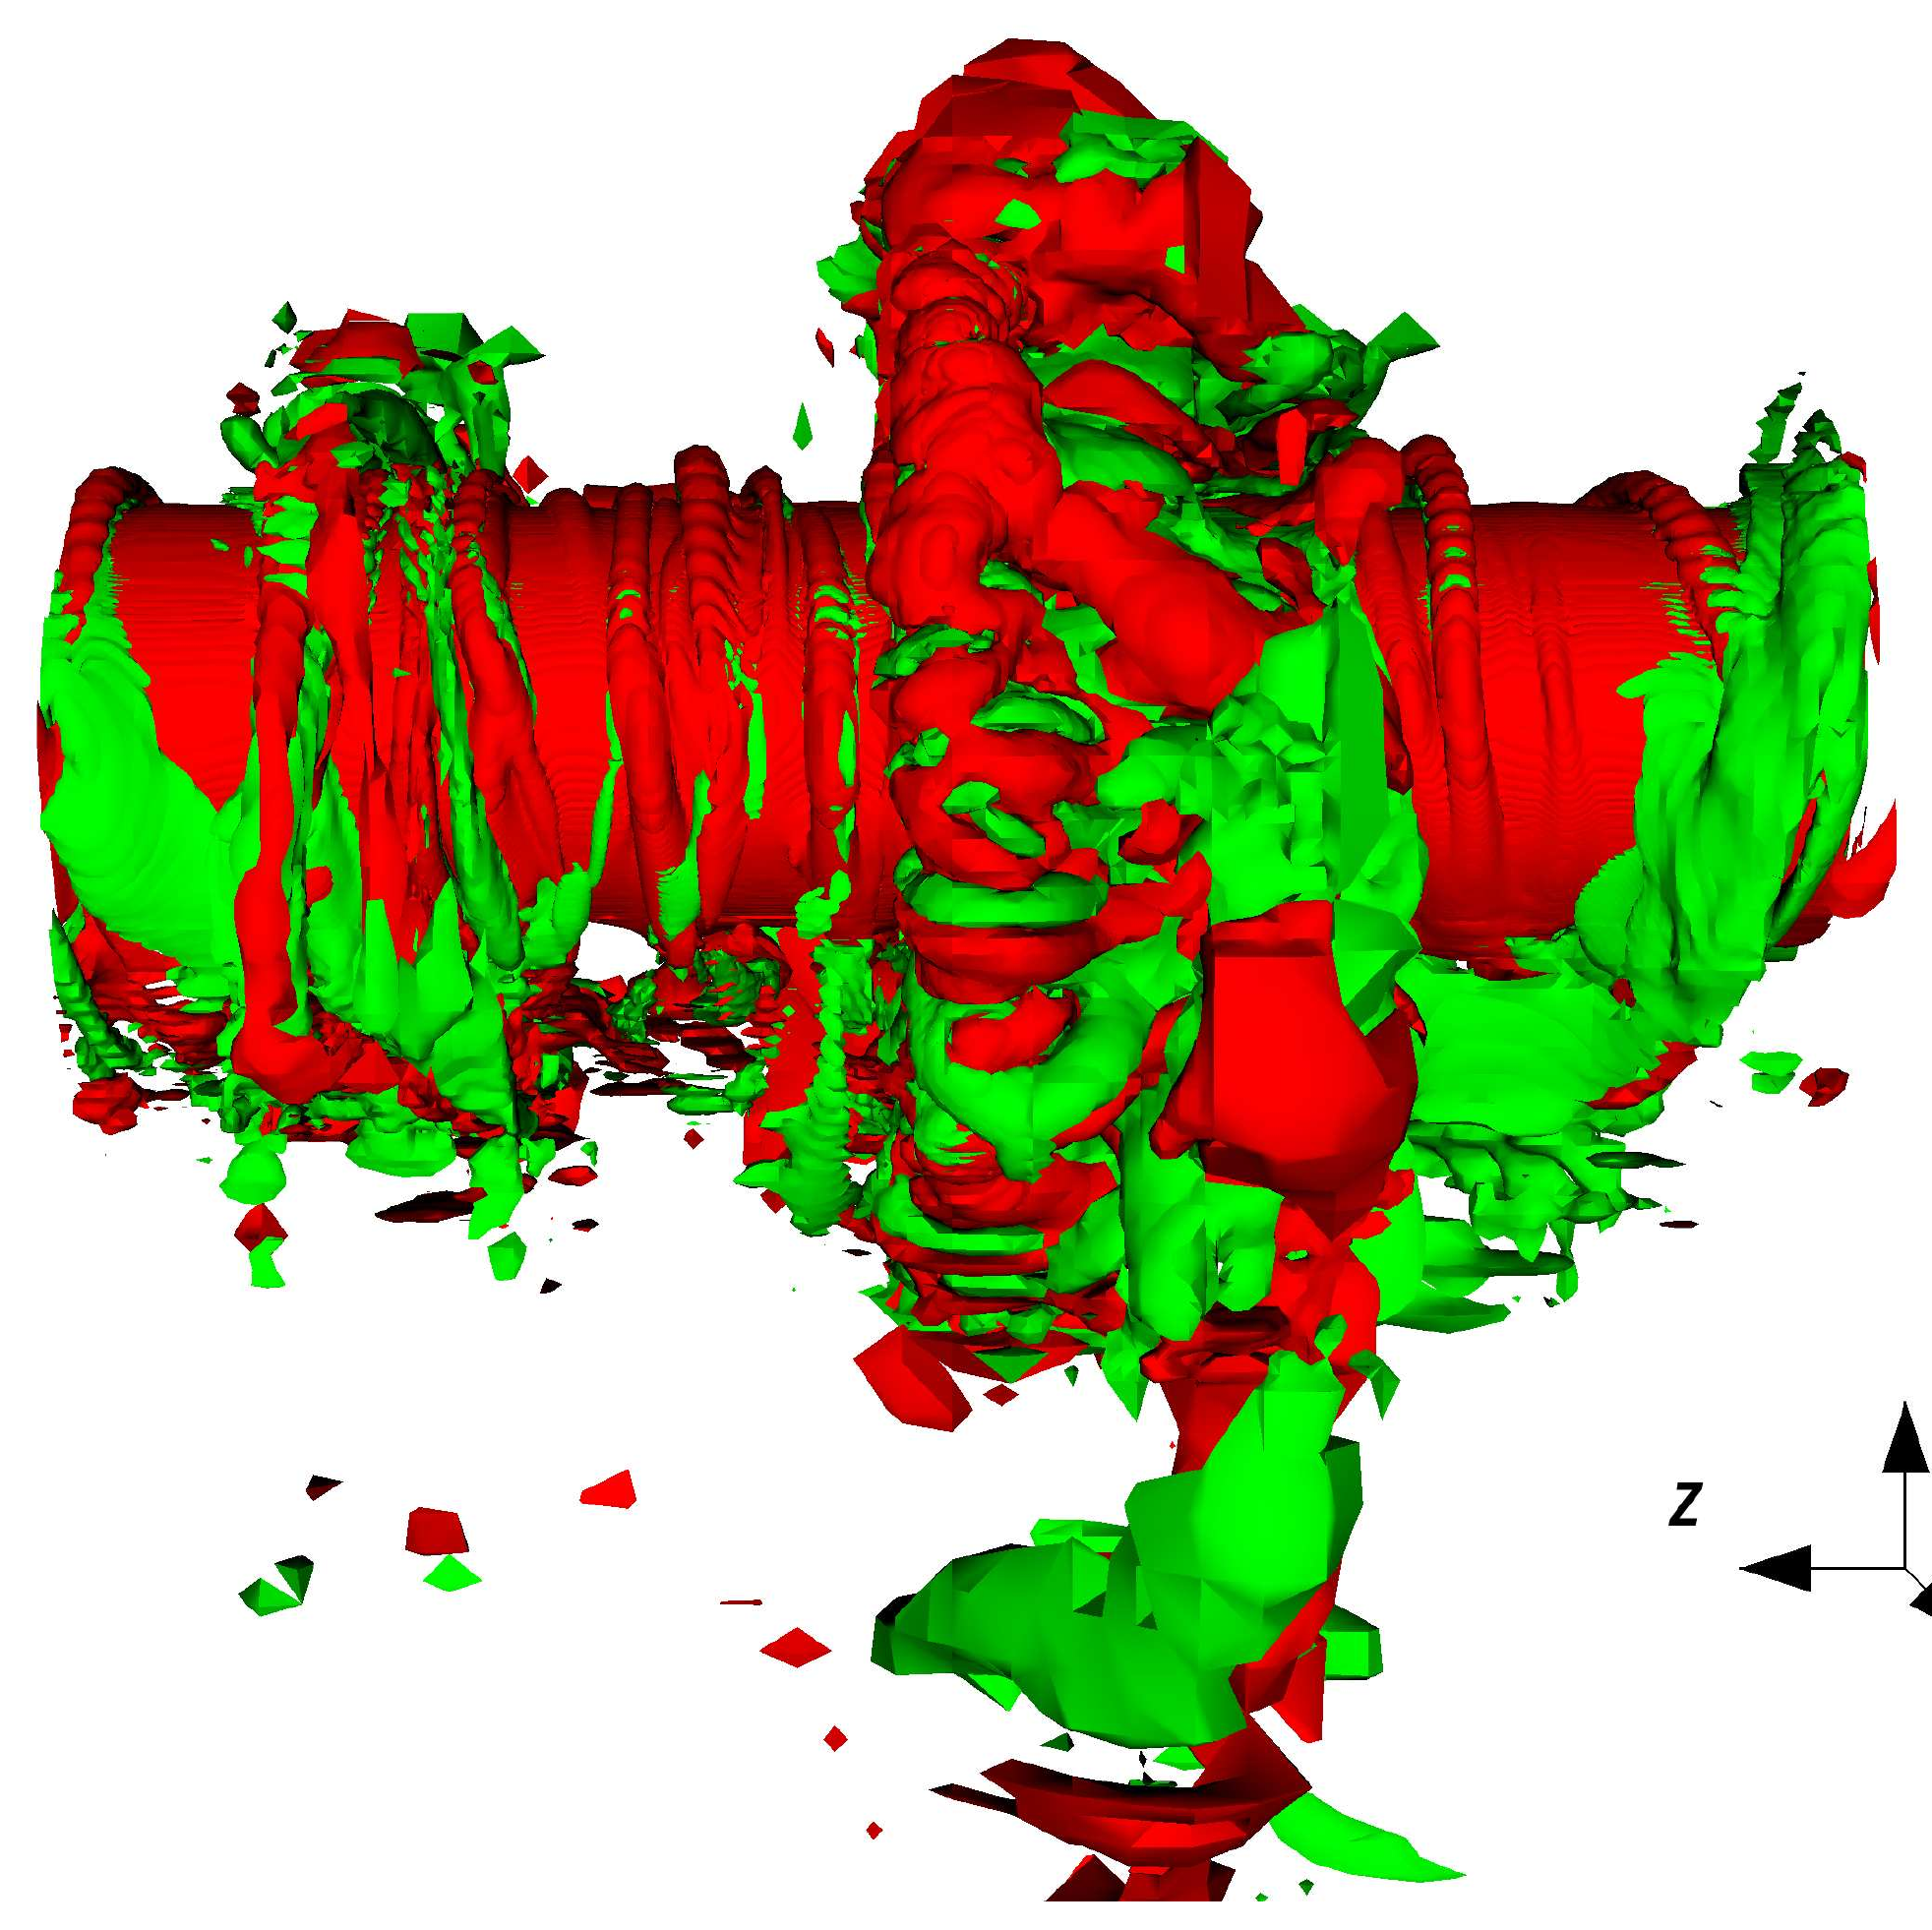
\includegraphics[width=\linewidth]{figures/faster_midfin_omega_z_t22_front.png}
  \caption{\texttt{faster\_midfin} (1 fin)}
\end{subfigure}
\caption{Same two cases and timestep as Figure~\ref{fig:tube}, viewed along
the streamwise direction (into the cross-flow / spanwise plane).}
\label{fig:front}
\end{figure}

\section{Open issues and next steps}

\begin{itemize}
  \item \textbf{Boundary ghost-cell crashes.} All three finned cases fail
  or stall near $x \approx 110$--$113$ from the same insufficient-ghost-cell
  error. A wider ghost-cell width for the IB spreading kernel, or simply
  stopping the run (or widening the domain) before the body reaches that
  region, is needed before any finned case can be compared cleanly out to
  $t = 30$ and beyond.
  \item \textbf{Incomplete glide-angle data for \texttt{faster\_midfin} and
  \texttt{faster\_2fin}.} Only \texttt{faster\_3fin} has a documented
  glide-angle progression; repeating that analysis for 1 and 2 fins is
  needed to say whether the flattening effect scales with fin count or is
  mostly a 0-vs-any-fins effect.
  \item \textbf{\texttt{faster\_nofin\_full\_span} also flattens, despite
  having no fins.} It ends in roughly the same $y$ band as the finned
  cases (Figure~\ref{fig:trajectories}), which could mean the fins are not
  the only thing driving the flattening (the longer, periodic-span body
  itself may matter), or could simply be an artifact of every one of these
  cases being cut off near the same $x$. Separating those two explanations
  needs either a full glide-angle time series for
  \texttt{faster\_nofin\_full\_span} (not currently committed) or runs that
  get past the current boundary stopping point.
  \item \textbf{Stale per-case documentation.} The \texttt{faster\_nofin\_full\_span}
  and \texttt{faster\_3fin} READMEs describe superseded, earlier runs; they
  should be refreshed from the latest completed/crashed run data to avoid
  the kind of cross-checking this report had to do against the case index.
  \item \textbf{\texttt{endcaps} is not a controlled comparison.} Its
  differing oscillation frequency, gravity onset, and boundary condition
  mean any difference from \texttt{faster\_nofin} cannot yet be attributed
  to the end caps alone.
\end{itemize}

\end{document}
